\documentclass[aspectratio=169]{beamer}
% SGSSS Beamer Preamble — shared across all lectures
% Brand colours from SGSSS logo

\usetheme{metropolis}

% --- Colour definitions ---
\definecolor{sgsssMagenta}{HTML}{A3217A}
\definecolor{sgsssGreen}{HTML}{2D6A3F}
\definecolor{sgsssBlack}{HTML}{1D1D1B}
\definecolor{sgsssWhite}{HTML}{FFFFFF}
\definecolor{sgsssLightGrey}{HTML}{F5F5F5}

% --- Metropolis colour overrides ---
\setbeamercolor{palette primary}{bg=sgsssMagenta, fg=sgsssWhite}
\setbeamercolor{title separator}{fg=sgsssGreen}
\setbeamercolor{progress bar}{fg=sgsssGreen, bg=sgsssLightGrey}
\setbeamercolor{frametitle}{bg=sgsssMagenta, fg=sgsssWhite}
\setbeamercolor{alerted text}{fg=sgsssMagenta}
\setbeamercolor{example text}{fg=sgsssGreen}
\setbeamercolor{block title}{bg=sgsssMagenta, fg=sgsssWhite}
\setbeamercolor{block body}{bg=sgsssLightGrey, fg=sgsssBlack}
\setbeamercolor{block title example}{bg=sgsssGreen, fg=sgsssWhite}
\setbeamercolor{block body example}{bg=sgsssLightGrey, fg=sgsssBlack}
\setbeamercolor{normal text}{fg=sgsssBlack}

% --- Fonts ---
\usepackage[T1]{fontenc}
\usepackage[sfdefault]{FiraSans}
\usepackage{FiraMono}
\setbeamerfont{frametitle}{size=\large}

% --- Packages ---
\usepackage{graphicx}
\usepackage{hyperref}
\usepackage{array}
\usepackage{booktabs}
\usepackage{minted}
\usepackage{fontawesome5}

% --- TikZ ---
\usepackage{tikz}
\usetikzlibrary{arrows.meta, positioning, shapes.geometric, trees, calc, decorations.pathmorphing, decorations.pathreplacing, fit, backgrounds}

% Reusable TikZ styles
\tikzset{
    server node/.style={rectangle, draw=sgsssGreen, fill=sgsssGreen!10, thick, minimum width=2.5cm, minimum height=1.2cm, align=center, font=\small},
    client node/.style={rectangle, draw=sgsssMagenta, fill=sgsssMagenta!10, thick, minimum width=2.5cm, minimum height=1.2cm, align=center, font=\small},
    api node/.style={rectangle, draw=sgsssGreen, fill=sgsssGreen!15, thick, rounded corners, minimum width=2.5cm, minimum height=1.2cm, align=center, font=\small},
    data node/.style={rectangle, draw=sgsssBlack, fill=sgsssLightGrey, thick, minimum width=2cm, minimum height=1cm, align=center, font=\small},
    arrow style/.style={-{Stealth[length=3mm]}, thick, sgsssBlack},
    html tag/.style={rectangle, draw=sgsssMagenta, fill=sgsssMagenta!8, rounded corners=2pt, font=\ttfamily\small, inner sep=4pt},
    json key/.style={rectangle, draw=sgsssGreen, fill=sgsssGreen!8, rounded corners=2pt, font=\ttfamily\small, inner sep=4pt},
}

% --- Minted configuration ---
\setminted{
    fontsize=\footnotesize,
    frame=leftline,
    framesep=2mm,
    baselinestretch=1.1,
    bgcolor=sgsssLightGrey,
    breaklines,
    linenos=false,
}
\setminted[python]{style=friendly}
\setminted[r]{style=friendly}

% --- Convenience commands ---
\newcommand{\pythoncode}[1]{\mintinline{python}{#1}}
\newcommand{\rcode}[1]{\mintinline{r}{#1}}
\newcommand{\httpstatus}[2]{\texttt{#1} \textit{#2}}

% --- Footer (page numbers only; logo on title slide only) ---
\setbeamertemplate{frame footer}{%
    \insertframenumber/\inserttotalframenumber%
}

% --- Metadata ---
\author{Dr Diarmuid McDonnell}
\institute{Braw Data Ltd \and Gradel Institute of Charity, University of Oxford}
\date{24 February 2026}


\title{What Are APIs and Why Use Them?}
\subtitle{Collecting Digital Data --- SGSSS Training Course}

\begin{document}

% -------------------------------------------------------
% Slide 1: Title
% -------------------------------------------------------
{
\setbeamertemplate{frame footer}{}
\begin{frame}[plain]
    \begin{center}
        \includegraphics[height=2.5cm]{../img/SGSSS_Stacked.png}\\[0.8cm]
        {\Large\bfseries\color{sgsssMagenta} Collecting Digital Data}\\[0.2cm]
        {\large What Are APIs and Why Use Them?}\\[0.6cm]
        {\normalsize Dr Diarmuid McDonnell}\\[0.1cm]
        {\small Braw Data Ltd \(\cdot\) Gradel Institute of Charity, University of Oxford}\\[0.3cm]
        {\small 24 February 2026}
    \end{center}
\end{frame}
}

% -------------------------------------------------------
% Slide 2: Section title
% -------------------------------------------------------
\section{What Are APIs and Why Use Them?}

% -------------------------------------------------------
% Slide 2: What is an API?
% -------------------------------------------------------
\begin{frame}{What is an API?}
    \begin{center}
    \begin{tikzpicture}[node distance=3cm]
        % Nodes
        \node[client node] (app) {\faIcon{laptop-code}\\Your Application};
        \node[api node, right=of app] (api) {\faIcon{exchange-alt}\\API};
        \node[server node, right=of api] (service) {\faIcon{database}\\Database/Service};

        % Arrows — Request (top) and Response (bottom)
        \draw[arrow style] ([yshift=0.4cm]app.east) -- ([yshift=0.4cm]api.west)
            node[midway, above, font=\small] {Request};
        \draw[arrow style] ([yshift=-0.4cm]api.west) -- ([yshift=-0.4cm]app.east)
            node[midway, below, font=\small] {Response};

        \draw[arrow style] ([yshift=0.4cm]api.east) -- ([yshift=0.4cm]service.west)
            node[midway, above, font=\small] {Query};
        \draw[arrow style] ([yshift=-0.4cm]service.west) -- ([yshift=-0.4cm]api.east)
            node[midway, below, font=\small] {Data};
    \end{tikzpicture}
    \end{center}

    \vspace{0.3cm}
    \textbf{API} = \textbf{A}pplication \textbf{P}rogramming \textbf{I}nterface

    \vspace{0.2cm}
    {\small Think of it as a \alert{translator}: your application doesn't need to know
    \emph{how} the database is organised --- it just asks the API in a standard way,
    and the API returns structured data.}
\end{frame}

% -------------------------------------------------------
% Slide 3: APIs vs web scraping
% -------------------------------------------------------
\begin{frame}{APIs vs Web Scraping}
    \centering
    \small
    \begin{tabular}{@{}l >{\raggedright\arraybackslash}p{4.5cm} >{\raggedright\arraybackslash}p{4.5cm}@{}}
        \toprule
        & \textbf{Web Scraping} & \textbf{APIs} \\
        \midrule
        \textbf{Data format}
            & Unstructured HTML
            & Structured JSON/XML \\[0.3em]
        \textbf{Reliability}
            & Breaks when site changes
            & Versioned, documented \\[0.3em]
        \textbf{Legality}
            & Grey area
            & Usually explicit ToS \\[0.3em]
        \textbf{Rate limits}
            & You must self-impose
            & Enforced by provider \\[0.3em]
        \textbf{Authentication}
            & Usually none
            & Often API key \\
        \bottomrule
    \end{tabular}

    \vspace{0.5cm}
    \begin{alertblock}{Rule of thumb}
        If an API exists, use it. Web scraping is a last resort.
    \end{alertblock}
\end{frame}

% -------------------------------------------------------
% Slide 4: Anatomy of an API call
% -------------------------------------------------------
\begin{frame}{Anatomy of an API Call}
    \begin{center}
    \begin{tikzpicture}[
        every node/.style={font=\small},
        brace/.style={decorate, decoration={brace, amplitude=5pt, raise=2pt}},
        label/.style={font=\footnotesize, align=center},
    ]
        % The full URL
        \node[anchor=west, font=\ttfamily\footnotesize] (url) at (0,0) {%
            \textcolor{sgsssGreen}{https://data.police.uk}%
            \textcolor{sgsssBlack}{/api/stops-force}%
            \textcolor{sgsssMagenta}{?force=city-of-london\&date=2024-01}%
        };

        % Braces and labels underneath
        \draw[brace, sgsssGreen] (0,-0.55) -- (3.55,-0.55)
            node[below=8pt, midway, label, text=sgsssGreen] {Base URL};
        \draw[brace, sgsssBlack] (3.55,-0.55) -- (6.35,-0.55)
            node[below=8pt, midway, label, text=sgsssBlack] {Endpoint};
        \draw[brace, sgsssMagenta] (6.35,-0.55) -- (12.65,-0.55)
            node[below=8pt, midway, label, text=sgsssMagenta] {Query parameters\\{\scriptsize key=value pairs joined by \&}};

        % Headers and Auth boxes
        \node[data node, below=2.5cm of url.west, anchor=west, minimum width=4.5cm] (headers) {%
            \faIcon{envelope}\;\textbf{Headers}\\[2pt]
            {\footnotesize\ttfamily Accept: application/json}%
        };
        \node[data node, right=1cm of headers, minimum width=4.5cm] (auth) {%
            \faIcon{key}\;\textbf{Authentication}\\[2pt]
            {\footnotesize API key, OAuth token, or none}%
        };
    \end{tikzpicture}
    \end{center}

    \vspace{0.1cm}
    {\small The UK Police API is \textbf{open} --- no authentication needed. Many other
    APIs require an API key sent as a header or query parameter.}
\end{frame}

% -------------------------------------------------------
% Slide 5: Reading API documentation
% -------------------------------------------------------
\begin{frame}{Reading API Documentation}
    \small
    \textbf{What to look for when you open the docs:}

    \vspace{0.15cm}
    \begin{itemize}\itemsep0pt
        \item[\textcolor{sgsssGreen}{\faIcon{check-circle}}] \textbf{Endpoints} --- what URLs are available and what data do they return?
        \item[\textcolor{sgsssGreen}{\faIcon{check-circle}}] \textbf{Authentication method} --- API key, OAuth, or open access?
        \item[\textcolor{sgsssGreen}{\faIcon{check-circle}}] \textbf{Rate limits} --- how many requests per minute/day?
        \item[\textcolor{sgsssGreen}{\faIcon{check-circle}}] \textbf{Response format} --- JSON, XML, CSV?
        \item[\textcolor{sgsssGreen}{\faIcon{check-circle}}] \textbf{Example requests \& responses} --- try them in a browser first!
    \end{itemize}

    \vspace{0.15cm}
    \begin{exampleblock}{UK Police API --- \texttt{data.police.uk/docs/}}
        \scriptsize
        \begin{itemize}\itemsep0pt
            \item[\textcolor{sgsssGreen}{\faIcon{check}}] Open access (no key needed)
            \item[\textcolor{sgsssGreen}{\faIcon{check}}] Returns JSON
            \item[\textcolor{sgsssGreen}{\faIcon{check}}] Rate limit: 15 requests per second
            \item[\textcolor{sgsssGreen}{\faIcon{check}}] Endpoints: stop-and-search, crimes, neighbourhoods, forces
        \end{itemize}
    \end{exampleblock}
\end{frame}

% -------------------------------------------------------
% Slide 6: JSON deep-dive
% -------------------------------------------------------
\begin{frame}{JSON Deep-Dive}
    \begin{columns}[T]
        \begin{column}{0.48\textwidth}
            \colorbox{sgsssLightGrey}{\parbox{0.92\textwidth}{\ttfamily\small
            \{\\
            \quad \textcolor{sgsssGreen}{"type"}: \textcolor{sgsssMagenta}{"Person"},\\
            \quad \textcolor{sgsssGreen}{"age\_range"}: \textcolor{sgsssMagenta}{"18-24"},\\
            \quad \textcolor{sgsssGreen}{"legislation"}: [\\
            \qquad \{\\
            \qquad\quad \textcolor{sgsssGreen}{"name"}: \textcolor{sgsssMagenta}{"John Doe"},\\
            \qquad\quad \textcolor{sgsssGreen}{"age"}: \textcolor{sgsssMagenta}{21}\\
            \qquad \}\\
            \quad ],\\
            \quad \textcolor{sgsssGreen}{"outcome"}: \textcolor{sgsssMagenta}{true}\\
            \}
            }}

            \vspace{0.3cm}
            {\footnotesize
            \textcolor{sgsssGreen}{\rule{0.8cm}{2pt}} Keys \quad
            \textcolor{sgsssMagenta}{\rule{0.8cm}{2pt}} Values}
        \end{column}
        \begin{column}{0.48\textwidth}
            {\small \textbf{JSON types:}}
            \begin{itemize}
                \footnotesize
                \item \textbf{Object} \texttt{\{\}} --- key-value pairs
                \item \textbf{Array} \texttt{[]} --- ordered list
                \item \textbf{String}, \textbf{Number}, \textbf{Boolean}, \textbf{null}
            \end{itemize}

            \vspace{0.3cm}
            {\small JSON is the most common format for API responses. Each record is a set of \textcolor{sgsssGreen}{\textbf{key}}--\textcolor{sgsssMagenta}{\textbf{value}} pairs. Values can be strings, numbers, booleans, arrays, or nested objects.}
        \end{column}
    \end{columns}
\end{frame}

% -------------------------------------------------------
% Slide 7: Next up
% -------------------------------------------------------
\begin{frame}{Next Up}
    \begin{center}
        {\Large \alert{Practical 2: UK Police API}}\\[0.5cm]
        \begin{itemize}
            \item Make your first API request (in a browser, then in code)
            \item Parse JSON responses into tabular data
            \item Explore stop-and-search data for a chosen police force
            \item Handle pagination and query parameters
        \end{itemize}
        \vspace{0.5cm}
        {\normalsize Open the \textbf{Practical 2} notebook in Google Colab\\(Python or R --- your choice!)}
    \end{center}
\end{frame}

\end{document}
